\chapter{Ambiente di Analisi}
Al fine di effettuare adeguate campagne di analisi, \`e stato progettato un ambiente che permetta l'osservazione non intrusiva del sistema descritto.\\*
In questo capitolo, si individuano e descrivono due differenti configurazioni di analisi:
\begin{itemize}
	\item Configurazione \emph{online}, atta a osservare il comportamento del sistema alle RUI;
	\item Configurazione \emph{offline}, atta a osservare esclusivamente il comportamento del modulo SFA con dati simulati o riprodotti dal campo.
\end{itemize} 
\section{Configurazioni}
\subsection{Configurazione Online}
Partendo dall'architettura nominale descritta nel capitolo 2, si osservano le seguenti modifiche:
\begin{itemize}
	\item \emph{Sensor Set} viene rimpiazzato da un PC in grado di interfacciarsi con la piattaforma di elaborazione dati attraverso una LAN;
	\item OBCU viene rimpiazzato dallo stesso PC.
\end{itemize}
Lo schema dell'architettura descritta \`e riportato in figura \ref{fig:hwtest}.
\begin{figure}
	\centering
	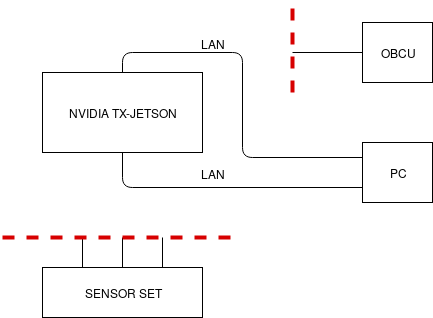
\includegraphics[width=0.7\linewidth]{img/hwtest}
	\caption{Configurazione \emph{online}}
	\label{fig:hwtest}
\end{figure}
\\*A livello di RUMI, i bus dati e il collegamento LTE sono stati rimpiazzati da una connessione LAN, ma permangono inalterate le interazioni ivi osservabili.\\*
Le modifiche descritte permettono di osservare variazioni nel comportamento del sistema quando sottoposto a campagne di \emph{fault injection}, simulando ad esempio guasti hardware nei bus dati, oppure perdite di segnale LTE.
\subsection{Configurazione Offline}
Questa modalit\`a di analisi prevede l'esecuzione del modulo SFA all'interno di un eseguibile \texttt{Windows}. Tale eseguibile prende il nome di \texttt{Rail Track Tool} (RTT), che include il modulo SFA come una classica dipendenza verso una libreria C++, sia essa \texttt{FusionLib}.\\*
\begin{figure}[h]
	\centering
	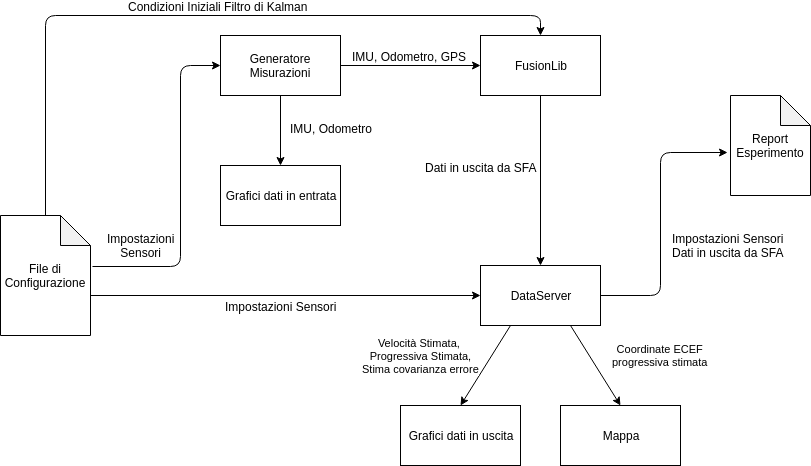
\includegraphics[width=0.9\linewidth]{img/rtt}
	\caption{Configurazione \emph{offline}}
	\label{fig:rtt}
\end{figure}\clearpage
Questa configurazione permette di valutare il comportamento di SFA al variare delle caratteristiche dei dati in ingresso, come ad esempio il numero di sensori abilitati o la covarianza del rumore insito nel processo di misura.